

\documentclass[12pt]{article}


\usepackage{graphicx}
\usepackage{subfig}
\usepackage{sidecap}
\usepackage{amsfonts}
\usepackage{amsmath}
\usepackage{amssymb}


\usepackage{psfrag}
%\usepackage{graphics}
\usepackage{float}

\usepackage{algorithm} 
\usepackage{algorithmic}
%\usepackage{algpseudocode}
\usepackage{epstopdf}

%\usepackage{showlabels}





%% For \bm (bold math)
\usepackage{bm}
\newcommand{\V}[1]{{\bm{\mathbf{\MakeLowercase{#1}}}}} % vector
\providecommand{\e}[1]{\ensuremath{\times 10^{#1}}}
\newcommand{\fraction}[2]{\textstyle\frac{#1}{#2}}
\newcommand{\Tr}{\textrm{Tr}}
\newcommand{\R}{\mathbb{R}}
\newcommand{\wkh}{\bar w_{k-L}^{k}}
\newcommand{\gkh}{\bar g_{k-L}^{k}}
\newcommand{\nh} {\widehat{\nabla}}
\newcommand{\wkb}{\bar{w}^k}
\newcommand{\gkb}{\bar{g}^k}
\newcommand{\wib}{\bar{w}^i}
\newcommand{\gib}{\bar{g}^i}
\newcommand{\bHV}{b_{\textrm{hv}}}
\newcommand{\bg}{\widehat{\nabla}F}
\newcommand{\Ss}{{\cal S}}
\newcommand{\Sh}{{\cal S}_H}
\newcommand{\N}{\mathbb{N}}
\newcommand{\bbh}{{b_H}}
\newcommand{\bb}{{b}}
\newcommand{\bM}{{M}}
\newcommand{\bL}{{L}}
%\newcommand{\bbh}{\boldsymbol{b_H}}
%\newcommand{\bb}{\boldsymbol{b}}
%\newcommand{\bM}{\boldsymbol{M}}
%\newcommand{\bL}{\boldsymbol{L}}


\def\NoNumber#1{{\def\alglinenumber##1{}\State #1}\addtocounter{ALG@line}{-1}}
\newcommand{\INDSTATE}[1][1]{\STATE\hspace{#1\algorithmicindent}}
\newcommand{\defeq}{\stackrel{\triangle}{=}}
\usepackage{soul,color}


%\usepackage{setspace}
%\usepackage{rotating}

\textwidth     =  6.0in
\textheight    =  8.2in
\oddsidemargin =  0.2in
\topmargin     = -0.4in


%margins
%\setlength{\paperwidth}{8.5in} \setlength{\paperheight}{11in}
%\setlength{\textwidth}{6in} \setlength{\textheight}{9in}
%\setlength{\oddsidemargin}{0in} \setlength{\evensidemargin}{0in} \setlength{\hoffset}{0in}
%\setlength{\topmargin}{0in} \setlength{\voffset}{0in} \setlength{\headheight}{0in} \setlength{\headsep}{0in} \setlength{\footskip}{30pt}%new types of headings
\newtheorem{theorem}{Theorem}[section]
\newtheorem{corollary}[theorem]{Corollary}
\newtheorem{lemma}[theorem]{Lemma}
\newtheorem{proposition}[theorem]{Proposition}
\newtheorem{problem}[theorem]{Problem}
\newtheorem{example}[theorem]{Example}
%\newtheorem{algorithm}[theorem]{Algorithm}
\newtheorem{definition}[theorem]{Definition}
\newtheorem{conjecture}[theorem]{Conjecture}
\newtheorem{question}[theorem]{Question}
\newtheorem{open}[theorem]{Open Problem}
\newtheorem{remark}[theorem]{Remark}
\newtheorem{claim}[theorem]{Claim}

\renewcommand{\theequation}{\thesection.\arabic{equation}}
\newcommand{\comment}[1]{}

\setcounter{section}{0}%

\begin{document}
% generates the title
\title{ Theory and Design of a Stochastic Quasi-Newton Method for Machine Learning}
\author{R. H. Byrd\thanks{Department of Computer Science, University of Colorado,
        Boulder, CO, USA.  This author was supported by National Science Foundation
        grant DMS-1216554 and Department of Energy grant DE-SC0001774.}
        \and 
       J. Nocedal \thanks{Department of Industrial Engineering and Management Sciences, Northwestern University, 
       Evanston, IL, USA.  This author was supported by National Science Foundation grant DMS-0810213, and by Department 
       of Energy grant DE-FG02-87ER25047.} 
       \and
       F. Oztoprak\thanks{Department of Engineering Sciences and Applied Mathematics, Northwestern University, 
       Evanston, IL, USA.  This author was supported by National Science Foundation grant DMS-0810213.} 
        \and   
        S. Solntsev \thanks{Department of Industrial Engineering and Management Sciences, Northwestern University, 
       Evanston, IL, USA.  This author was supported by National Science Foundation grant DMS-0810213, and by Department 
       of Energy grant DE-FG02-87ER25047.}
      }
%****

\maketitle
\begin{abstract}{ It has recently been shown that stochastic quasi-Newton methods can be effective for solving large-scale
learning problems. The algorithm described in \cite{sammy} employs the limited memory BFGS method, defining the curvature vectors in a way that controls noise. Many of the properties of that algorithm remained unexplored. In this paper, we present an advanced implementation of the algorithm that is suitable for both convex and nonconvex problems.
}
\end{abstract}
\newpage


\section{Agenda}
\label{agenda}

\begin{enumerate}
\item Theory of Stochastic Quasi-Newton Methods
\begin{enumerate}
	\item It would be nice to be the first to develop realistic convergence analysis for the stochastic quasi-Newton iteration
	\begin{equation}
	         x_{k+1}= x_k - \alpha H_k \widehat \nabla f(x_k)    \label{qn}
	 \end{equation}
	  Murata considers $H_k = H^*$ and Bottou and LeCun $H_k \rightarrow H*$.  Suppose Dennis-More' condition holds; what
	     can we prove (see paper by Ribeiro \cite{mokhtariregularized})? Ultimately it would be interesting to study the complete
	     algorithm with the interaction between $H_k$ and the step.
	  	\item When should one employ the covariance matrix or the Hessian? Should the algorithm be built on the Natural Gradient
	        method?  What is the relationship between
	         iteration \eqref{qn} and the idealized version of AdaGrad that keeps a full matrix?  How about the incremental 
	         Gauss-Newton method of Bertsekas (which Bach suggested as an alternative to what we do)? \textcolor{blue}{ it
	         appears that the natural gradient method does not have anything for us to offer at this stage (i.e. before we
	         deal with neural nets)}\textcolor{red}{Action: Stefan will write a summary of the Schraudolph paper as an Appendix
	         to the krakoy document}
	         	\end{enumerate}         
\item Design of Stochastic Quasi-Newton Methods
\begin{enumerate}
	\item Develop a mature version of
	        the stochastic quasi-Newton method in Sammy's paper.
	\begin{enumerate}
		\item Experiments with small batches $b=1,2, 5$ \textcolor{blue}{done}
		\item RCV1 is the wrong problem (according to Bottou). Add one ore more test problems.
		\item Try algorithm with constant steplength \textcolor{blue}{in progress}
		\item Compare with AdaGrad and possibly with incremental Gauss Newton.
		\item Idealized experiments (\textcolor{blue}{Stefan advocates this}). Use the exact Hessian at each iteration 
		         or the LeRoux matrix or the
		         full AdaGrad matrix.
		         These are small scale experiments in which matrices are inverted.
		\item  Refinements of Sammy's method. How should $s$ be defined?
		          Memory issues in the limited memory approach and  coordination between $L$ and $b_H$.
		          \textcolor{blue}{Richard advocates this}
		\item Frank variation (described below). Explain why it is unlikely to improve upon current approach.
		\item Consider a stochastic Newton-CG method. Do operation counts, write document arguing why
		         it is less attractive than stochastic QN. \textcolor{blue}{Jorge will write}
		\item How should one sample for Hessian-vector products? Yoram suggests oversampling and then
		         choosing the terms with a high classification error. How can the memory parameter $M$ vary during
		         the course of the iteration? Relationship with theory of random matrices.
		 \item Develop Neural Nets version (non-convex) using Gauss-Newton matrix. Is line search appropriate
		          in this context? Need collaborators: Google or IBM? Or perhaps Microsoft via Bottou.
     \end{enumerate}  
     \item Second order information in stochastic averaging methods like SAG?
	\begin{enumerate}
	\item Can one design averaging methods that benefit from second order information? 
	  Numerical results for Bach-Moulines are given at the end of this document. Lin Xiao advocates a different method; see 
	         xiao-progressive in the karakoy/reading file
	         	 \item Fishing Methods. A description of the method is given in section \ref{fishing}
	 	\end{enumerate}   
\end{enumerate}
\end{enumerate}



%%%%
\section{Introduction}
\label{formulation}

This paper discusses the design and analysis of  a quasi-Newton method that operates in
the stochastic approximation regime. Building on the  algorithm proposed in \cite{sammy}, we introduce a 
series of modifications and extensions that make the algorithm more versatile, dependent on a fewer number of
parameters, and better suited for producing robust generalization results.

The problem under consideration is the minimization of a convex stochastic
function, 
\begin{equation}  \label{ff}  
     \min_{w \in \R^n} F(w)   =  \mathbb{E} [f(w; \xi)]  ,
\end{equation}
where $\xi$ is a random variable. Although problem \eqref{ff} arises other in
settings, such as simulation optimization \cite{asmussen2007stochastic}, we assume for concreteness that $\xi$
is a random instance consisting of an input-output pair $(x,z)$. The vector
$x$ is typically referred to in machine learning as the input representation while $z$ as the
target output. In this setting, $f$ typically takes the following form
%to an example (data-point) from
%a predefined space ${\cal X}$.
\begin{equation}   \label{pp}
  f(w; \xi)= f(w;x_i, z_i) = \ell (h(w; x_i); z_i),
\end{equation}
where $\ell$ is a loss function into $\R_+$ and $h$ is a
prediction model, parametrized by $w$. The collection of input-output
pairs $\{(x_i, z_i)\}$, $i = 1,\cdots,N$ is often referred to as the
training set. The objective function \eqref{ff} is defined using the empirical
expectation 
\begin{equation} \label{empirical}
        F(w) = \frac{1}{N}\sum_{i=1}^N f(w;x_i, z_i).
\end{equation}
In learning applications with massive amounts for training data, it is
often mandatory to use a stochastic gradient based on $b \defeq |\Ss| \ll N$
input-output
instances, yielding the following estimate
\begin{equation}   \label{bat}
\bg(w) = \frac{1}{b} \sum_{i \in \Ss}  \nabla f(w;x_i, z_i) ~.
\end{equation}
The subset $\Ss$ $\subset \{ 1, 2, \cdots, N\}$ is randomly chosen, with 
$b $ sufficiently small so that the algorithm operates in the stochastic
approximation regime. Therefore, the stochastic estimates of the gradient are
substantially faster to compute than a gradient based on the entire  training set.

The algorithm proposed in \cite{sammy} employs the well known
limited memory BFGS updating formula~\cite{LiuNocedal89}, and
show how to collect second-order information that is reliable enough to
produce stable and productive Hessian approximations. The key is to compute
average curvature estimates at regular intervals using (sub-sampled)
Hessian-vector products. This ensures sample uniformity and
avoids the potentially harmful effects of differencing noisy gradients.  



The iterations in the algorithm given in \cite{sammy} are of the form
\begin{equation}   \label{rm}
   w^{k+1} = w^k - \alpha^k B_k^{-1} \bg(w^k) ~,
\end{equation}
where $B_k$ is a symmetric positive definite approximation to the Hessian
matrix $\nabla^2 F(w)$, and $\alpha^k>0$.  In our experiments, the steplength
parameter $\alpha^k$ has the form $\alpha^k = \beta/k$, where $\beta >0$ is
given, but other choices can be employed.
 
%In applications involving a large amount of noisy data, it is often efficient to replace $\widetilde \nabla F(w^k)$, which is based on only one {\color{blue} random instance}, with an average of $b$ gradient samplings. We use the notation
% \begin{equation}   \label{bat}
%         \bg(w^k) = \frac{1}{b} \sum_{i=1}^b  \nabla f(w^k;\xi^i)
% \end{equation}
%to denote a mini-batch gradient, with the understanding that $b$ is small enough so that iteration \eqref{rm} operates in the stochastic approximation regime.

% @@@@@@

A critical question is how to construct $B_k$ in a stable manner. Furthermore, to make each iteration scalable, the algorithm must be able to update the inverse matrix $H_k= B_k^{-1}$ directly, so that \eqref{rm} can be implemented as
\begin{equation}   \label{direct}
        w^{k+1} = w^k - \alpha^k H_k \bg(w^k) .
 \end{equation}
 This step computation should require only $O(n)$ operations, as in limited memory quasi-Newton methods for deterministic optimization. 

If we set $H_k=I$ and $\alpha^k= \beta/k$ in \eqref{direct}, we recover the classical Robbins-Monro method \cite{RobMon51}, which is also called the \emph{stochastic gradient descent method}. Under standard assumptions, the number of iterations needed by this method to compute an $\epsilon$-accurate solution is 
\[
      \frac{\nu\kappa^2}{\epsilon} + O\left(\frac{1}{\epsilon}\right) ,
 \] 
 where $\kappa$ is the condition number of the Hessian at the optimal solution, $\nabla^2 F(w^*)$, and $\nu$ is a parameter that depends on both the Hessian matrix and the gradient covariance matrix; see \cite{murata1998statistical,BottouBosq08}. Therefore, the stochastic gradient descent method is adversely affected by ill conditioning in the Hessian. In contrast, it is shown by Murata \cite{murata1998statistical} that setting $H_k=\nabla^2F(w^*)^{-1}$ in \eqref{direct}
completely removes the dependency of $\kappa$ from the complexity estimate. % $\frac{\nu}{\epsilon} + O\left(\frac{1}{\epsilon}\right)$.
Although the choice $H_k=\nabla^2 F(w^*)^{-1}$ is not viable in practice, it suggests that an appropriate choice of $H_k$ may result in an algorithm that improves upon the stochastic gradient descent method.

%In section~\ref{sec:qn} We
Byrd, Hansen, Nocedal and Singer \cite{sammy} presented a stochastic quasi-Newton method of the form \eqref{direct} that is designed for large-scale applications. It employs the limited memory BFGS method, which is defined in terms of \emph{correction pairs} $(s, y)$ that provide an estimate of the curvature of the objective function $F(w)$ along the most recently generated directions. We propose a novel way of defining these correction pairs that yields curvature estimates that are not corrupted by the effect 
of differencing the noise in the gradients. Their numerical experiments, using problems arising in machine learning, suggest that the new method is robust and efficient.

In this paper we consider again some of the building blocks of that algorithm and design a variant that improves upon it in various respects

The paper is organized into 5 sections. The new algorithm is presented in section~\ref{sec:qn}, and in section~\ref{numerical} we describe a set of experiments to illustrate its practical performance. 
%A discussion of the cost and implementation of the algorithm is given in section~\ref{discuss}. 
A literature survey on  related stochastic quasi-Newton methods is given in section~\ref{related}. The paper concludes in section~\ref{final} with some remarks about the contributions of the paper, and with some open questions.
 
\bigskip\noindent\emph{Notation.}  

\section{Extension of Bottou-Le Cun Theory}
\label{ext}

Using the machinery in the paper "A Tool for the Analysis of Quasi-Newton Methods with Application to Unconstrained 
Minimization (1989), SIAM J. Numerical Analysis, 26, 3, pp. 727-739, with R. Byrd." to prove the following result.

Consider the BFGS method that updates the Hessian approximation every L iterations. The objective function is deterministic.
\section{Comparison with AdaGrad}
\label{adagrad}
In this section we compare the numerical performance of AdaGrad and the stochastic BFGS method (SQN). We consider both the diagonal version of AdaGrad and the full matrix version which is similar to the incremental Gauss-Newton method.

The diagonal version of AdaGrad is given as follows:

\begin{algorithm}[H]
\caption{AdaGrad (Original Version)}
\label{ada1}
\begin{algorithmic}[1]
\REQUIRE  $\eta>0$ $\delta \geq 0$
\STATE  $k=0$ $s_{-1}=0$
\WHILE{$x^k$ doesn't satisfy stopping condition}   
\STATE $s_{k,i} =\sqrt{   \sum_{j=1}^k g_{j,i}^2   }  =\sqrt{ ((k-1) s_{k-1,i})^2 +g_{k,i}^2 }, \quad i=1, \cdots, n  $
\STATE $H_k =\delta I + diag(s_k)$
\STATE $x^{k+1} = x^k - \eta H_k^{-1} g_k$
\STATE $k=k+1$
\ENDWHILE
\end{algorithmic}
\end{algorithm}

Note that there is no need to store the previous gradients. As indicated in Step~3, the update to $s_k$ can be done recursively. A quote from the AdaGrad paper concerning the choice of $\delta$: ``concretely, for some small fixed $\delta \geq 0$  (specified later, though in practice $\delta$ can be set to 0)'' I am not sure how true this is. To quote again from the AdaGrad paper: `` there is no need to keep track of a learning rate as in previous algorithms, as it is implicitly given by the growth of the proximal function''. [By this they probably mean that one does not have to chose from $1/k, 1/\sqrt{k}$ etc.] It is important to stress that the parameter $\eta$ needs to be tuned.

For the experiments, we reorganized the AdaGrad iteration a bit, so that the constant $\eta$ in AdaGrad is comparable to the constant $\beta$ in SQN. The implemented version is as follows:



\bigskip
\begin{algorithm}[H]
\caption{AdaGrad (Implemented Version)}
\label{ada2}
\begin{algorithmic}[1]
\REQUIRE  $\eta>0$ $\delta \geq 0$
\STATE  $k=0$ $s_{-1}=0$
\WHILE{$x^k$ doesn't satisfy stopping condition}   
\STATE $s_{k,i} = \frac{1}{k} \sqrt{   \sum_{j=1}^k g_{j,i}^2   }  =\frac{1}{k} \sqrt{ ((k-1) s_{k-1,i})^2 +g_{k,i}^2 }, \quad i=1, \cdots, n  $
\STATE $H_k= \frac{\delta I}{k} + diag(s_k)$
\STATE $x^{k+1} = x^k - \frac{\eta}{k} H_k^{-1} g_k$
\STATE $k=k+1$
\ENDWHILE
\end{algorithmic}
\end{algorithm}


We test on the same problems used in Sammy's paper. Results are shown for a range of values of $\eta$ in Algorithm~\ref{ada1}, which are labeled as {\tt a} in the Figures.

\begin{figure}[H] 
 \centering
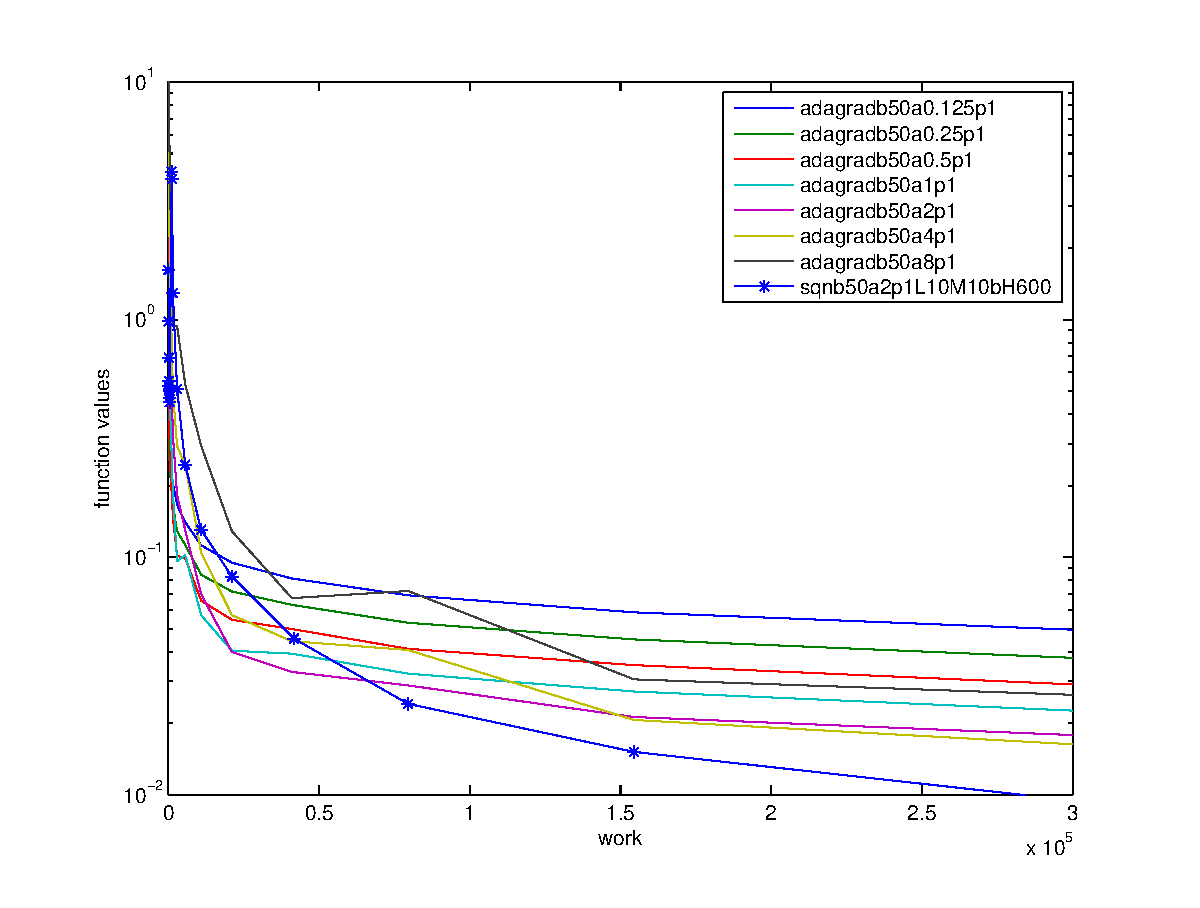
\includegraphics[scale=1]{Stefan/paperOnImpFigures/yoram-adagrad.eps}
\caption{{\bf Synthetic dataset}. Illustration of SQN and AdaGrad. A gradient batch size {\tt b=50} is used in all runs. (Ignore the parameter {\tt p}). AdaGrad was implemented as in Algorithm~\ref{ada1}; the parameter $\eta$ is indicated by {\tt a}. For SQN we used the same parameters as in Sammy's paper. (It is not clear that they are optimal for this problem, but we can use them as a benchmark.) The 1 on the horizontal axis corresponds to 14 epochs for Adagrad}
\label{yoram1}
\end{figure}

The results in Figure~\ref{yoram1} indicate that AdaGrad is faster at the beginning, but SQN overtakes it 10 epochs or so. 


\begin{figure}[H] 
 \centering
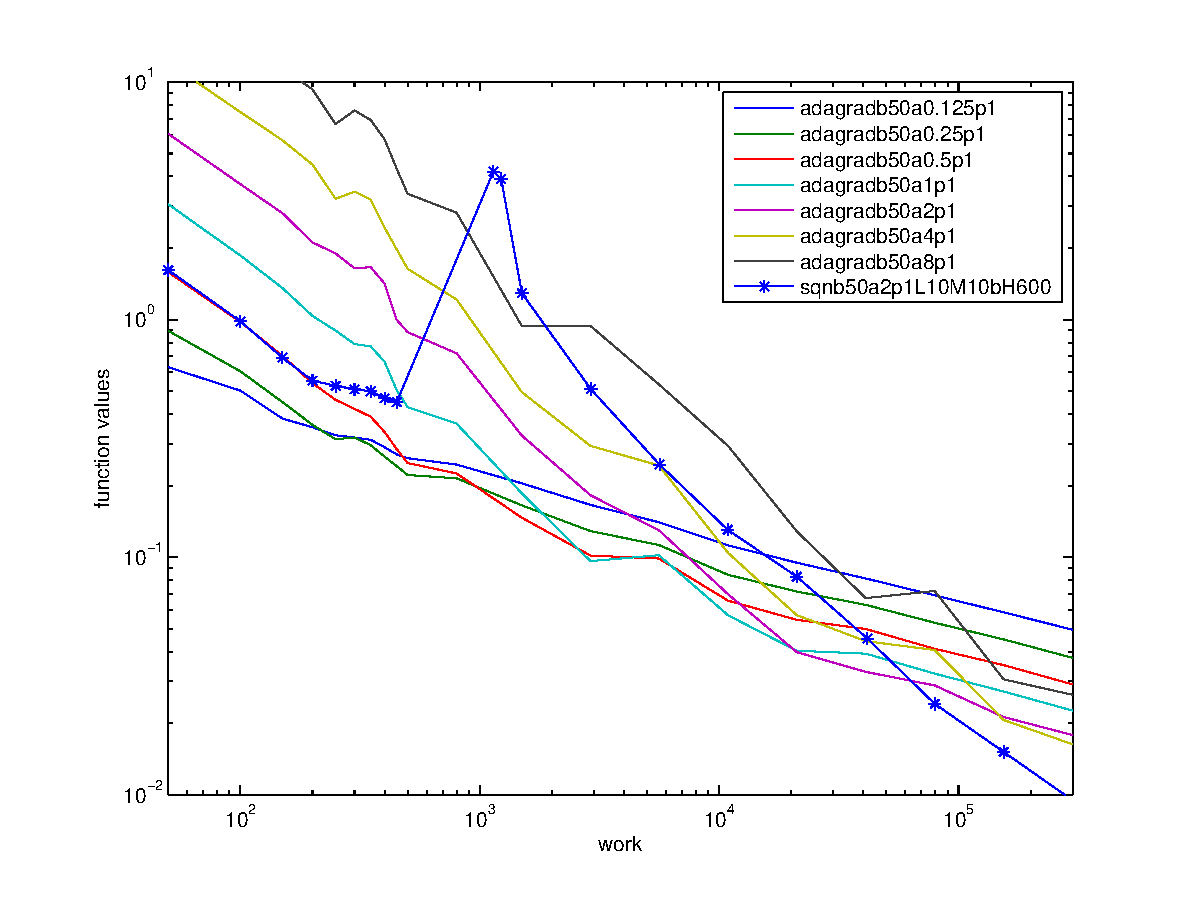
\includegraphics[scale=1]{Stefan/paperOnImpFigures/yoram-adagrad-l.eps}
\caption{{\bf Synthetic dataset} Same results as in Figure~\ref{yoram1} but using a logarithmic scale in the x-axis}
\label{yoram2}
\end{figure}


Next we consider the Speech problem
\begin{figure}[H] 
 \centering
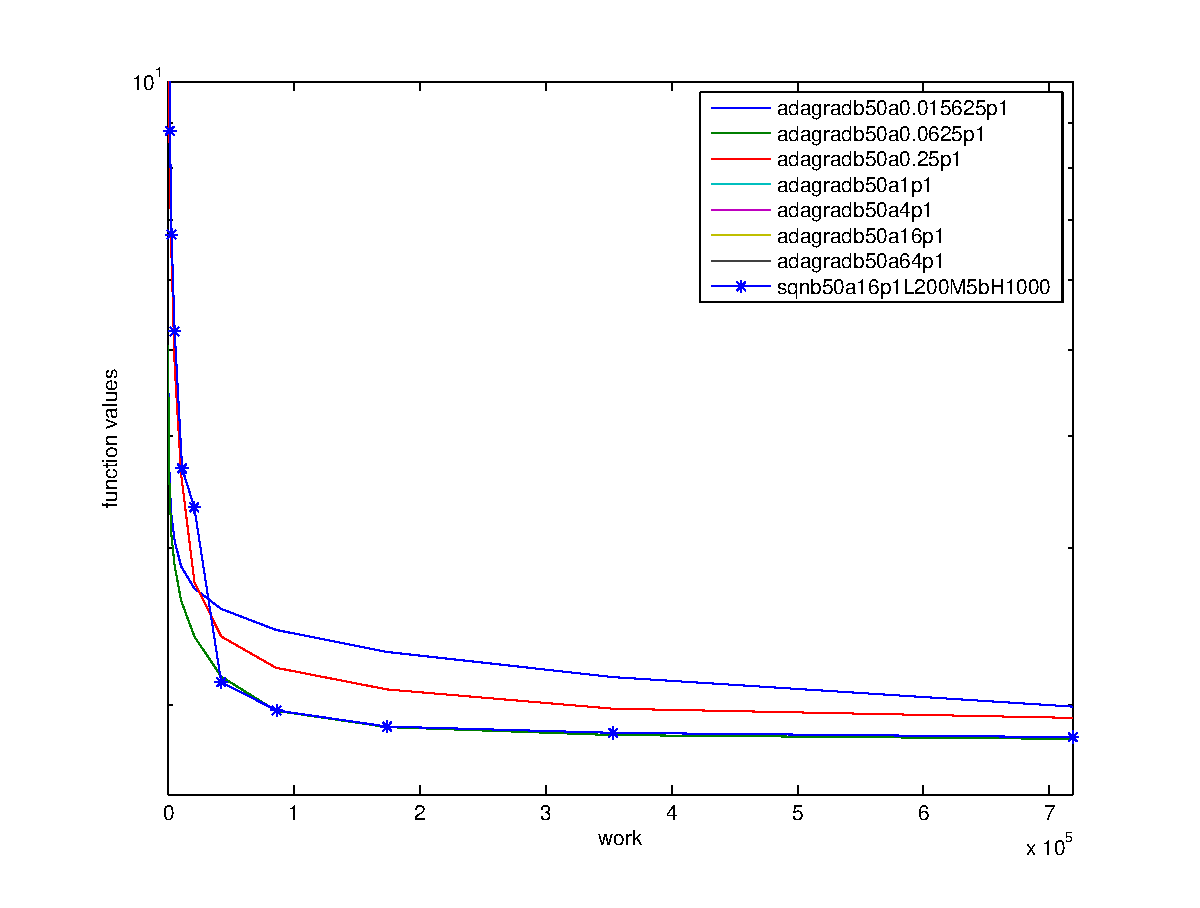
\includegraphics[scale=1]{Stefan/paperOnImpFigures/speech-adagrad.eps}
\caption{{\bf Speech dataset} The 1 on the vertical axis corresponds to half an epoch}
\label{speech1}
\end{figure}


\begin{figure}[H] 
 \centering
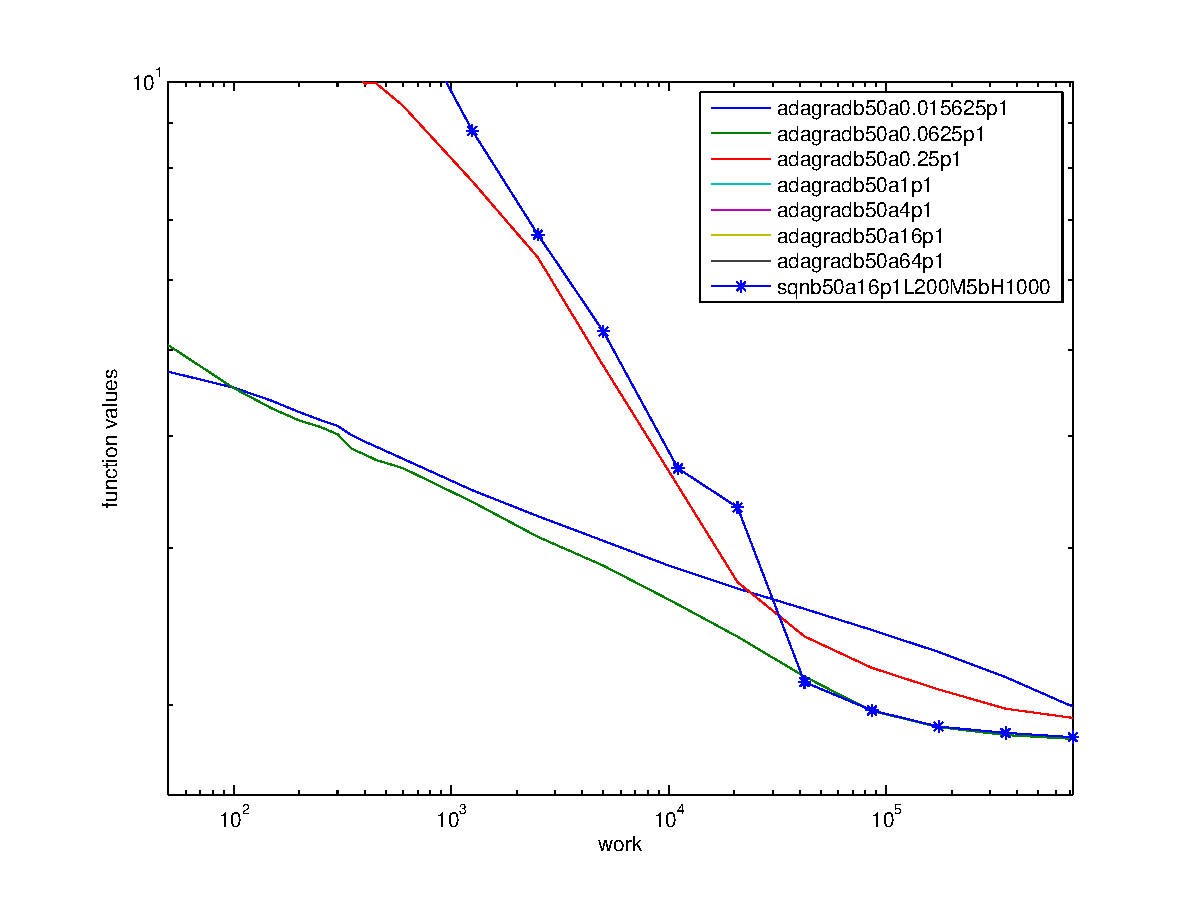
\includegraphics[scale=1]{Stefan/paperOnImpFigures/speech-adagrad-l.eps}
\caption{{\bf Speech dataset} Same results as in Figure~\ref{speech1} but using a logarithmic scale}
\label{speech2}
\end{figure}






\section{New Data Sets}
\label{data}
Action Items
\begin{enumerate}
\item Stefan to look at the {\\t tf-idf } version of RCV1. Do we know how to define the objective function? See the paper by Shalev-Schwartz
\item Jorge to discuss with Alekh if the new RCV1 file is good for testing second-order methods
\item Understand Yoram's random problem generator. Compare the code with the description in paper [8] referenced in Sammy's paper
\end{enumerate}
Our first task is for all of us to understand well the random problem generator by Yoram. He says that he has used it to test codes before that are used in production systems.

Alekh Agarwal (a colleague of Bottou at Microsoft) also mentioned that RCV1 is the wrong problem for our tests. He suggests
the MNIST and CIFAR datasets, and the feature selection is described in the appendix of one of the papers he sent; see agarwal-1.pdf and agarwal-2.pdf in the karakoy/reading file. 

Summary of email exchange
\begin{verbatim}
As promised, I am sending you an email with our paper on using batch-second
order methods for some large-scale prediction problems. The MNIST and 
CIFAR datasets used here are fairly standard, and the feature construction 
is all described in the appendix. Let me know if you would like some of our 
code for feature generation. The paper can be found at 
http://arxiv.org/pdf/1310.1949v2.
I also wanted to mention our other paper on distributed machine learning 
which I briefly mentioned, where we show that initializing a Quasi-Newton 
method with a SGD solution can have substantial speedups in distributed 
settings. That paper is available at http://arxiv.org/abs/1110.4198.
\end{verbatim}


\section{Covariance vs Hessian}
\label{covariance}

We begin by considering a fundamental question: should our algorithm be based on the Natural Gradient of Amari, or on
the unscaled gradient of the objective function. Furthermore, should the quasi-Newton formula approximate the covariance or the Hessian matrix, and of what function?

\subsection{Amari, LeRoux}
\textcolor{blue}{Figen comments of 2/22/14}
I think I can now put in words the point of the figure I was drawing on the whiteboard today (data-function-parameter).

I think the question I had in my mind was the following: In a quasi-Newton method, we accumulate some useful information about the geometry of the function we minimize.  In a stochastic setting, our observations are not purely on the rate of change in the gradient of the function, but we also make observations on the noise in those evaluations.  Can't it then be useful to accumulate some information about the character of that random noise as we proceed?

To make it more concrete, suppose we have two matrices at each iteration, an approximation H to the Hessian, and an estimation C to the variance of the noise term $\xi$.  Each update of H is rank two, and each update of C is rank one ($\xi_k$'s has independent identical distribution with zero mean).  The two updates support each other: given a noisy measurement $g_k$ of the gradient at $x_k$, $H(x_k-x)$ provides an approximation $y_k$ so that we can use $(g_k-y_k)$ to update C; on the other hand, scaling $g_k$ with the inverse of $C^{-1/2}$, we can get an estimate $t_k$ of $g_k$ with reduced variance and use $t_k$ to update H.  Finally, we can use $H^{-1}$ to scale $t_k$, and move from $x_k$ to a new solution point.

The above scenario assumes that the decision variables of the optimization problem are different from the parameters of the probability distribution of measurement errors.  When they are the same (as in a maximum likelihood problem), minimizing f is equivalent to learning the distribution -- perhaps we can then work with a single matrix.  I did not yet think about that.
\textcolor{blue}{End of Figen comments of 2/22/14}


\subsection{Bengio Paper}



\textcolor{blue}{Figen Comments of 3/25/14:} I also read the paper.  I think the problem definition here is a little bit more specific than the one we have been considering so far: The decision variables $\theta$ are the parameters of the probability distribution of the input data z. (However, the loss function that defines the objective is not necessarily the log likelihood).  According to the derivation of the natural gradient in Section 2, which is based on model problem (3), the natural gradient step is first order in terms of objective function minimization (it does not scale the gradient using the Hessian of the objective), but second order in terms of constraint violation minimization (second order approximation to the trust-region-like constraint of (3) is employed in (5)) if I understand everything correctly.  I am not sure if I understood well the 'Hessian on the manifold' mentioned in Section 9 (i.e. they do not formally state it but describe it as the Hessian of the error as a function of the probability density functions $p_\theta$).

In our last call I have been talking about employing the covariance matrix because I have been considering the more general scenario where the variables of optimization and the parameters of the probability distribution of the noise are not the same.  I have been thinking that the covariance matrix could help with scaling the step with respect to the geometry of the noise, while the Hessian does so with respect to the geometry of the objective as usual.  (For a while I thought the 'score function' mentioned in Section 4 of the Polyak-Juditski paper can be relevant to this but I am still not sure.)


PS. I am almost done studying the analysis in Polyak-Juditski paper; the way they prove the asymptotic distribution is very different than the lines of the analysis we have seen in the Murata paper.  (I know they analyze different algorithms but I believe that a similar analysis to the one in P-J paper could be considered for the pure stochastic gradient algorithm).

\textcolor{blue}{End Figen's comments of 3/25/14}

\section{AdaGrad, Incremental Gauss-Newton and LeRoux methods}
\label{ada}

 
$\sigma^2$ is the covariance of the prior distribution on $g$, $m$ is the number of datapoints, $\hat{g}$ is the sample gradient. 

The precise algorithm is as follows. We assume $C(\cdot)$ is the true covariance matrix of the gradients, and computable by 
\begin{equation}
	C(\theta) = \int_x \left( \frac{\partial L(\theta,x)}{\partial \theta}-g\right) \left(\frac{\partial L(\theta,x)}{\partial \theta}-g \right)^T p(x) dx
\end{equation}

\begin{algorithm}[H]
\caption{Natural Gradient - Ideal version}
\label{alg1}
\begin{algorithmic}[1]
\REQUIRE  $\alpha_k$, $C(\cdot)$, $\hat{g}(\cdot)$, $x^0$
\STATE  $k=0$
\WHILE{$x^k$ doesn't satisfy stopping condition}   
\STATE $x^{k+1} = x^k - \alpha_k \left[ I +  \frac{C(x^k)}{m \sigma^2}\right]^{-1} \hat{g}(x^k)$
\STATE $k=k+1$
\ENDWHILE
\end{algorithmic}
\end{algorithm}

The algorithm below requires an approximation to the covariance to be constructed at each iteration. 
\begin{equation}
	\hat{C(\theta)} = \frac{1}{m} \sum_i \left( \frac{\partial L(\theta,x_i)}{\partial \theta}-g\right) \left(\frac{\partial L(\theta,x_i)}{\partial \theta}-g \right)^T
\end{equation}

\begin{verbatim}
Hi Francis,
After my talk, I believe that you asked: why not define the matrix as
       B <-- B + F'(xk)*F'(xk)^T
and use the Sherman Morrison formula to get the inverse? Initialize
            B=  delta*I

Is that what you suggested?

Hi Jorge,
This is exactly it, and this looks a lot like a Kalman filter / incremental 
Gauss-Newton method.

Hi Francis,
The thing is this: the Sherman-Morrison formula requires d^2 operations, so 
I don't see how this scales to large problems (unless one uses only the 
diagonal or something like that).

On the other hand limited memory BFGS method requires O(d) operations, so it 
scales well.

Hi Jorge.
If you store n gradients in dimension d in a matrix G, you can choose to do 
the inversion of (GG^\top + I) in O(d^2 n + d^3) or O(d n^2 +n^3). If n is small,
 the O(dn^2+n^3) can be advantageous. From my understanding, n is corresponds to 
 the limited memory in Quasi-Newton methods.
\end{verbatim}


\section{Limited Memory Approach}
\label{memory}

The behavior of the stochBFGS method was somewhat surprising in that increasing the memory in L-BFGS updating
improved performance substantially at first, but only marginally later. We want to understand if this is a generic property of
machine learning problems. [Bottou mentioned that we should not test rcv1].

It is also interesting investigate if it is possible to do an intelligent selection of the sample points used in Hessian-vector products.

\section{Hessian Cost vs Gradient Cost}
\label{coordinate}

The stochBFGS method has too many parameters, which may prevent it from becoming widely used. Two parameters, BHV and L are clearly related, so in this section we investigate them.

For a given amount of work, balance bHV and L. To be specific, fix the batch size b; then vary bHV and L. There may be a reasonable answer on how to coordinat these parameters.

\section{The Nonconvex Case}
\label{nonconvex}

{\tt Action Items}. Stefan should talk to Sammy about her knowlege of deep learning, the discussions she had with Martens, and write a short summary here. Jorge will contact Martens co-author to see the state of affairs with their Hessian-free method.

The stochBFGS algorithm presented in \cite{sammy} is designed for the (strictly) convex case. Here we discuss how to apply the
method to problems such as those arising in deep learning, where the objective function is (highly) non-convex.

\section{Working with Small Batch Sizes}
\label{smallb}

The iteration costs given in section suggest that the stochBFGS method is not likely to be competitive with SG when the batch size is less than 10. It also remains to be shown that that algorithm is stable for b=1. 

\textcolor{blue}{These results have been done by Stefan}. They are very positive --- in fact counter-intuitive. Preliminary results with a fixed steplength are totally different: the advantage of the QN approach is no longer apparent.

\section{Variants Based on Averaging}
\label{averaging}

Several interesting algorithm have been proposed recently that lie somewhere in between stochastic and batch methods. They update a running average of the gradients computed so far, and update them in a random manner that yields a linear rate of convergence. A prototypical example is given by the SAG method of LeRoux, Schmidt and Bach.

 In this section we investigate how to design quasi-Newton methods based on this kind of information. As in the previous sections, it is crucial to maintain sample uniformity so that quasi-Newton approximations are not corrupted by noise.
 
 
\subsection{Fishing Methods}   \label{fishing}
This method attempts a single 

\begin{algorithm}[H]
\caption{Fishing Method}
\label{alg1}
\begin{algorithmic}[1]
\REQUIRE  $\gamma$, $x^0$, oracles to compute gradients and HV products at each datapoint
\STATE  $k=0$
\STATE  $\bar{x}^0 = x^0$
\WHILE{$x^k$ doesn't satisfy stopping condition  }   
\STATE Choose a random $h$, a datapoint
\STATE $x^{k+1} = x^k - \gamma (\nabla f_h(\bar{x}^k) + \nabla^2 f_h(\bar{x}^k) (x^k - \bar{x}^k))$
\STATE $\bar{x}^{k+1} = \frac{k\bar{x}^k +  x^{k+1}}{k+1}$
\STATE $k=k+1$
\ENDWHILE
\STATE $x^{END} = x^k - \gamma ((\nabla^2)^{-1} f_h(\bar{x}^k) \nabla f_h(\bar{x}^k) (x^k)$
\end{algorithmic}
\end{algorithm}
 
 \section{Numerical Results}
\label{numerical}

{\tt Action Item}. Select two other test problems. Keep rcv1 and compare. Bottou suggest using a random generator (like Yoram's) and forcing the problem to be increasingly more ill conditioned.

In this section we compare the algorithms presented in the previous sections with AdaGrad, SAG and the method proposed in \cite{sammy}. Our tests are divided into four parts.

First, we consider purely stochastic methods that employ a decaying steplength (learning rate).

Next, we consider the effect of using fixed steplengths in purely stochastic methods.

Next we compare semi-stochastic methods, like SAG. Here we employ constant stepsizes.

Finally, we perform experiments in the batch setting as a way to verify that the algorithms we propose reduce to efficient methods in the deterministic setting.



%%%%%%%%%%%%%%%%%%%%%%%%
\section{Final Remarks}   \label{final}
%%%%%%%%%%%%%%%%%%%%%%%%
In this paper, we presented a quasi-Newton method that operates in the stochastic approximation regime. It is designed for the minimization of convex stochastic functions, and was tested on problems arising in machine learning. In contrast to previous attempts at designing stochastic quasi-Newton methods, our approach does not employ differences of gradients, but gathers curvature information pointwise, and feeds this information into the BFGS formula, which is entrusted with the task of computing an inverse Hessian approximation. 


Our numerical results suggest that the method does more than rescale the gradient, i.e., that  its improved performance over the stochastic gradient descent method of Robbins-Monro is the result of incorporating curvature information in the form of a full (i.e. non-diagonal) matrix. 
 
 
The practical success of the algorithm relies on the fact that the batch size $b_{\rm hv} $ for Hessian-vector products can be chosen large enough to provide useful curvature estimates, while the update spacing $L$ can be chosen large enough (say $L= 20$) to amortize the cost of Hessian-vector products, and make them affordable.
Similarly, there is a wide range of values for the gradient batch size $b$ that makes the overall quasi-Newton approach (\ref{direct}) viable.
 

The use of the Hessian-vector products \eqref{newcor2} may not be essential; one might be able to achieve the same goals using differences in gradients, as in \eqref{cor:gradDiff}. 
This would require, however, the evaluation of gradients in \eqref{cor:gradDiff} using the same batch so as to obtain sample uniformity, as well as the development of a strategy to prevent close gradient differences from magnifying round off noise. In comparison, the use of Hessian-vector products takes care of these issues automatically, but it imposes the (slightly) onerous demand of requiring code for Hessian-vector computations.


The convergence analysis of our algorithm will be the subject of a separate study. That analysis must consider the delicate interaction between noisy gradients and noisy Hessian approximations. As in any quasi-Newton method, the analysis is intrinsically complex, as the Hessian approximation influences the iterates computed by the algorithm, and these iterates in turn influence the quasi-Newton update. The generation of poor curvature estimates must be controlled, with high probability, as quasi-Newton updating is an overwriting process, and the effect of bad updates can be quite harmful. 

Our numerical results suggest that the method presented in this paper holds much promise for the solution of large-scale problems arising in stochastic optimization.

%%%%%%%%%%%%%%%%%%%%%%%%
\section{Appendix 1: Email exchange with Bach}   \label{bach}
%%%%%%%%%%%%%%%%%%%%%%%%


 
 
%%%%%%%%%%%%%%%%%%%%%%%%
\section{Appendix 2: Survey by Guanghui Lang}   \label{bach}
%%%%%%%%%%%%%%%%%%%%%%%%

You briefly mentioned to me and asked if I can provide a list of recently developed/improved optimization algorithms that might be useful for machine learning. I found this seemed to be a difficult task as there is a lot of active research going on in this field. So I decided to list is a few stochastic and deterministic algorithms that I am familiar with (at least I read the referred papers). I hope that you do not mind that this list is definitely incomplete and maybe biased.

I put all these methods under the umbrella of huge-scale optimization.

\centerline{\large Huge-scale Optimization}

Iterative, lower-order, scalable to very large-scale problems.

\bigskip

Stochastic optimization:
\begin{itemize}
\item Stochastic mirror descent method (Nemirovski, Juditsky, Lan and Shapiro, 09).
\item Stochastic accelerated gradient methods (Lan 09,12), and its variant using dual averaging (Xiao 10).
\item Stochastic Quasi-Newton Methods (Nocedal et al. 11, 14).
\item Nonconvex stochastic gradient methods (Ghadimi and Lan 13).
\item Randomized coordinate descent methods (Nesterov 10, Richt\'{a}rik and Tak\'{a}c 12) and its stochastic
variant (Dang and Lan 13).
\end{itemize}

Deterministic first-order methods: 
\begin{itemize}
\item Low rank method for semidefinite programming (Burer, Monteiro and Zhang 02).
\item Smooth minimization of nonmooth problems (Nesterov 05), and the following related
algorithms for solving saddle-point/variational inequality problems.
\begin{itemize}
\item Mirror-prox method (Nemirovski 04). 
\item Primal-dual methods (Chambolle and Pork 11) and its accelerated version (Chen, Lan and Ouyang 13).
\item Alternating direction of multipliers (e.g., Boyd et. al. 11, Ouyang et al. 14).
\end{itemize}
\item Composite optimization with a smooth plus simple nonsmooth component (Nesterov 07, Tseng 08, Beck and Teboulle 09).
\item Uniformly optimal or parameter-free methods 
\begin{itemize}
\item Accelerated prox-level methods (Lan 10,11).
\item Universal gradient methods (Nesterov 13).
\end{itemize}
\item Linear optimization based or conditional gradient methods (Jaggi 13, Juditsky and Nemirovski 13, Lan 13).
\end{itemize}


 

\newpage
\small
\bibliographystyle{plain}

\bibliography{../References/references}
\end{document}

%%%%%%%%%%%%%%%%%%%%%%%%%%%%%%%%%%%%%%%%%%%%%%%%%%%%%%%%%%%%%

